% ルンゲ関数のチェビシェフ補間による比較図

\begin{figure}[H]
  \centering
  \caption{$f(x) = \frac{1}{1+25x^2}$のチェビシェフ補間（$n=4$次多項式）}
  \label{fig:runge-chebyshev-first}
  \vspace{5pt}
  \begin{minipage}[b]{0.48\linewidth}
    \centering
    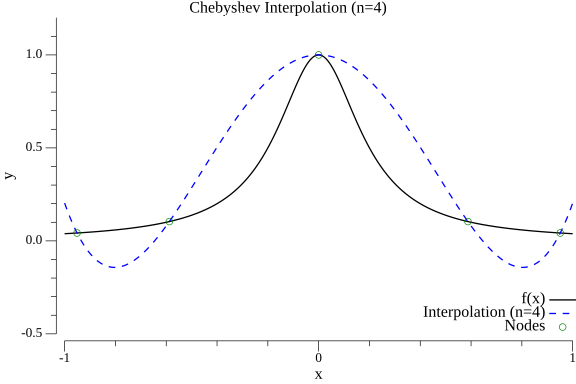
\includegraphics[width=1.0\linewidth]{material/runge/chebyshev/runge_cheby_n04.png}
  \end{minipage}
  \hfill
  \begin{minipage}[b]{0.48\linewidth}
    \centering
    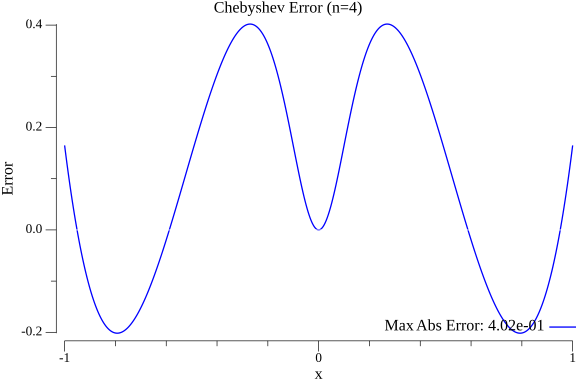
\includegraphics[width=1.0\linewidth]{material/runge/chebyshev/runge_cheby_err_n04.png}
  \end{minipage}
\end{figure}

\begin{figure}[H]
  \centering
  \caption{$f(x) = \frac{1}{1+25x^2}$のチェビシェフ補間（$n=7$次多項式）}
  \label{fig:runge-chebyshev-2}
  \vspace{5pt}
  \begin{minipage}[b]{0.48\linewidth}
    \centering
    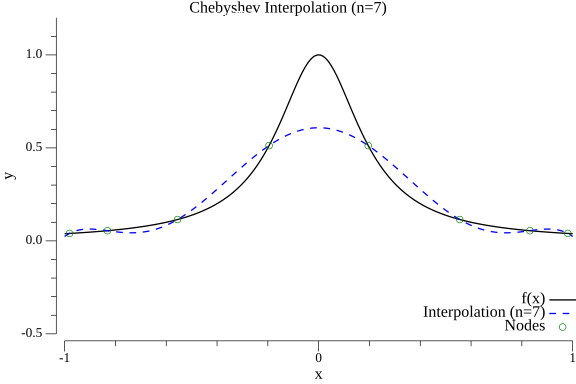
\includegraphics[width=1.0\linewidth]{material/runge/chebyshev/runge_cheby_n07.png}
  \end{minipage}
  \hfill
  \begin{minipage}[b]{0.48\linewidth}
    \centering
    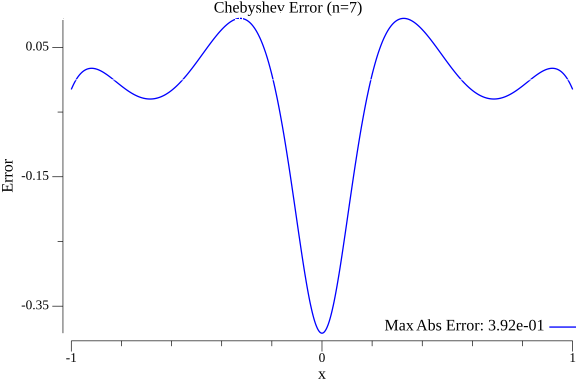
\includegraphics[width=1.0\linewidth]{material/runge/chebyshev/runge_cheby_err_n07.png}
  \end{minipage}
\end{figure}

\begin{figure}[H]
  \centering
  \caption{$f(x) = \frac{1}{1+25x^2}$のチェビシェフ補間（$n=15$次多項式）}
  \label{fig:runge-chebyshev-last}
  \vspace{5pt}
  \begin{minipage}[b]{0.48\linewidth}
    \centering
    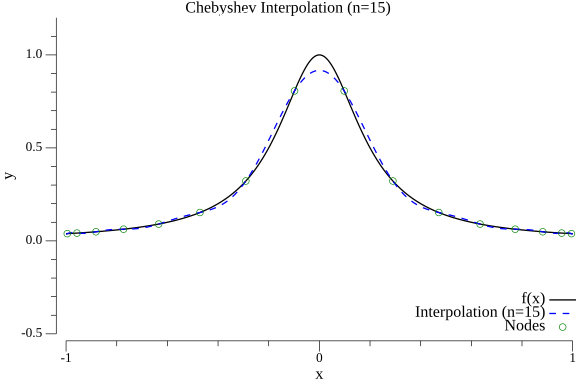
\includegraphics[width=1.0\linewidth]{material/runge/chebyshev/runge_cheby_n15.png}
  \end{minipage}
  \hfill
  \begin{minipage}[b]{0.48\linewidth}
    \centering
    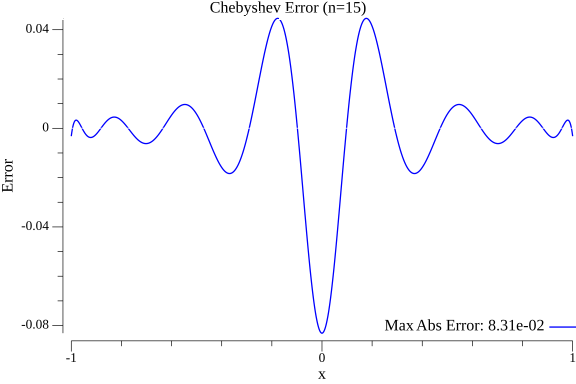
\includegraphics[width=1.0\linewidth]{material/runge/chebyshev/runge_cheby_err_n15.png}
  \end{minipage}
\end{figure}

